\documentclass{article}
\usepackage{tikz}
\usepackage{layouts}
\usepackage{geometry}
\geometry{letterpaper, hmargin=1cm, vmargin=1cm}
\def\numberHorizontal{18}
\def\numberVertical{25.5}
\def\mmm{*1.5mm}
\begin{document}

\pagestyle{empty}
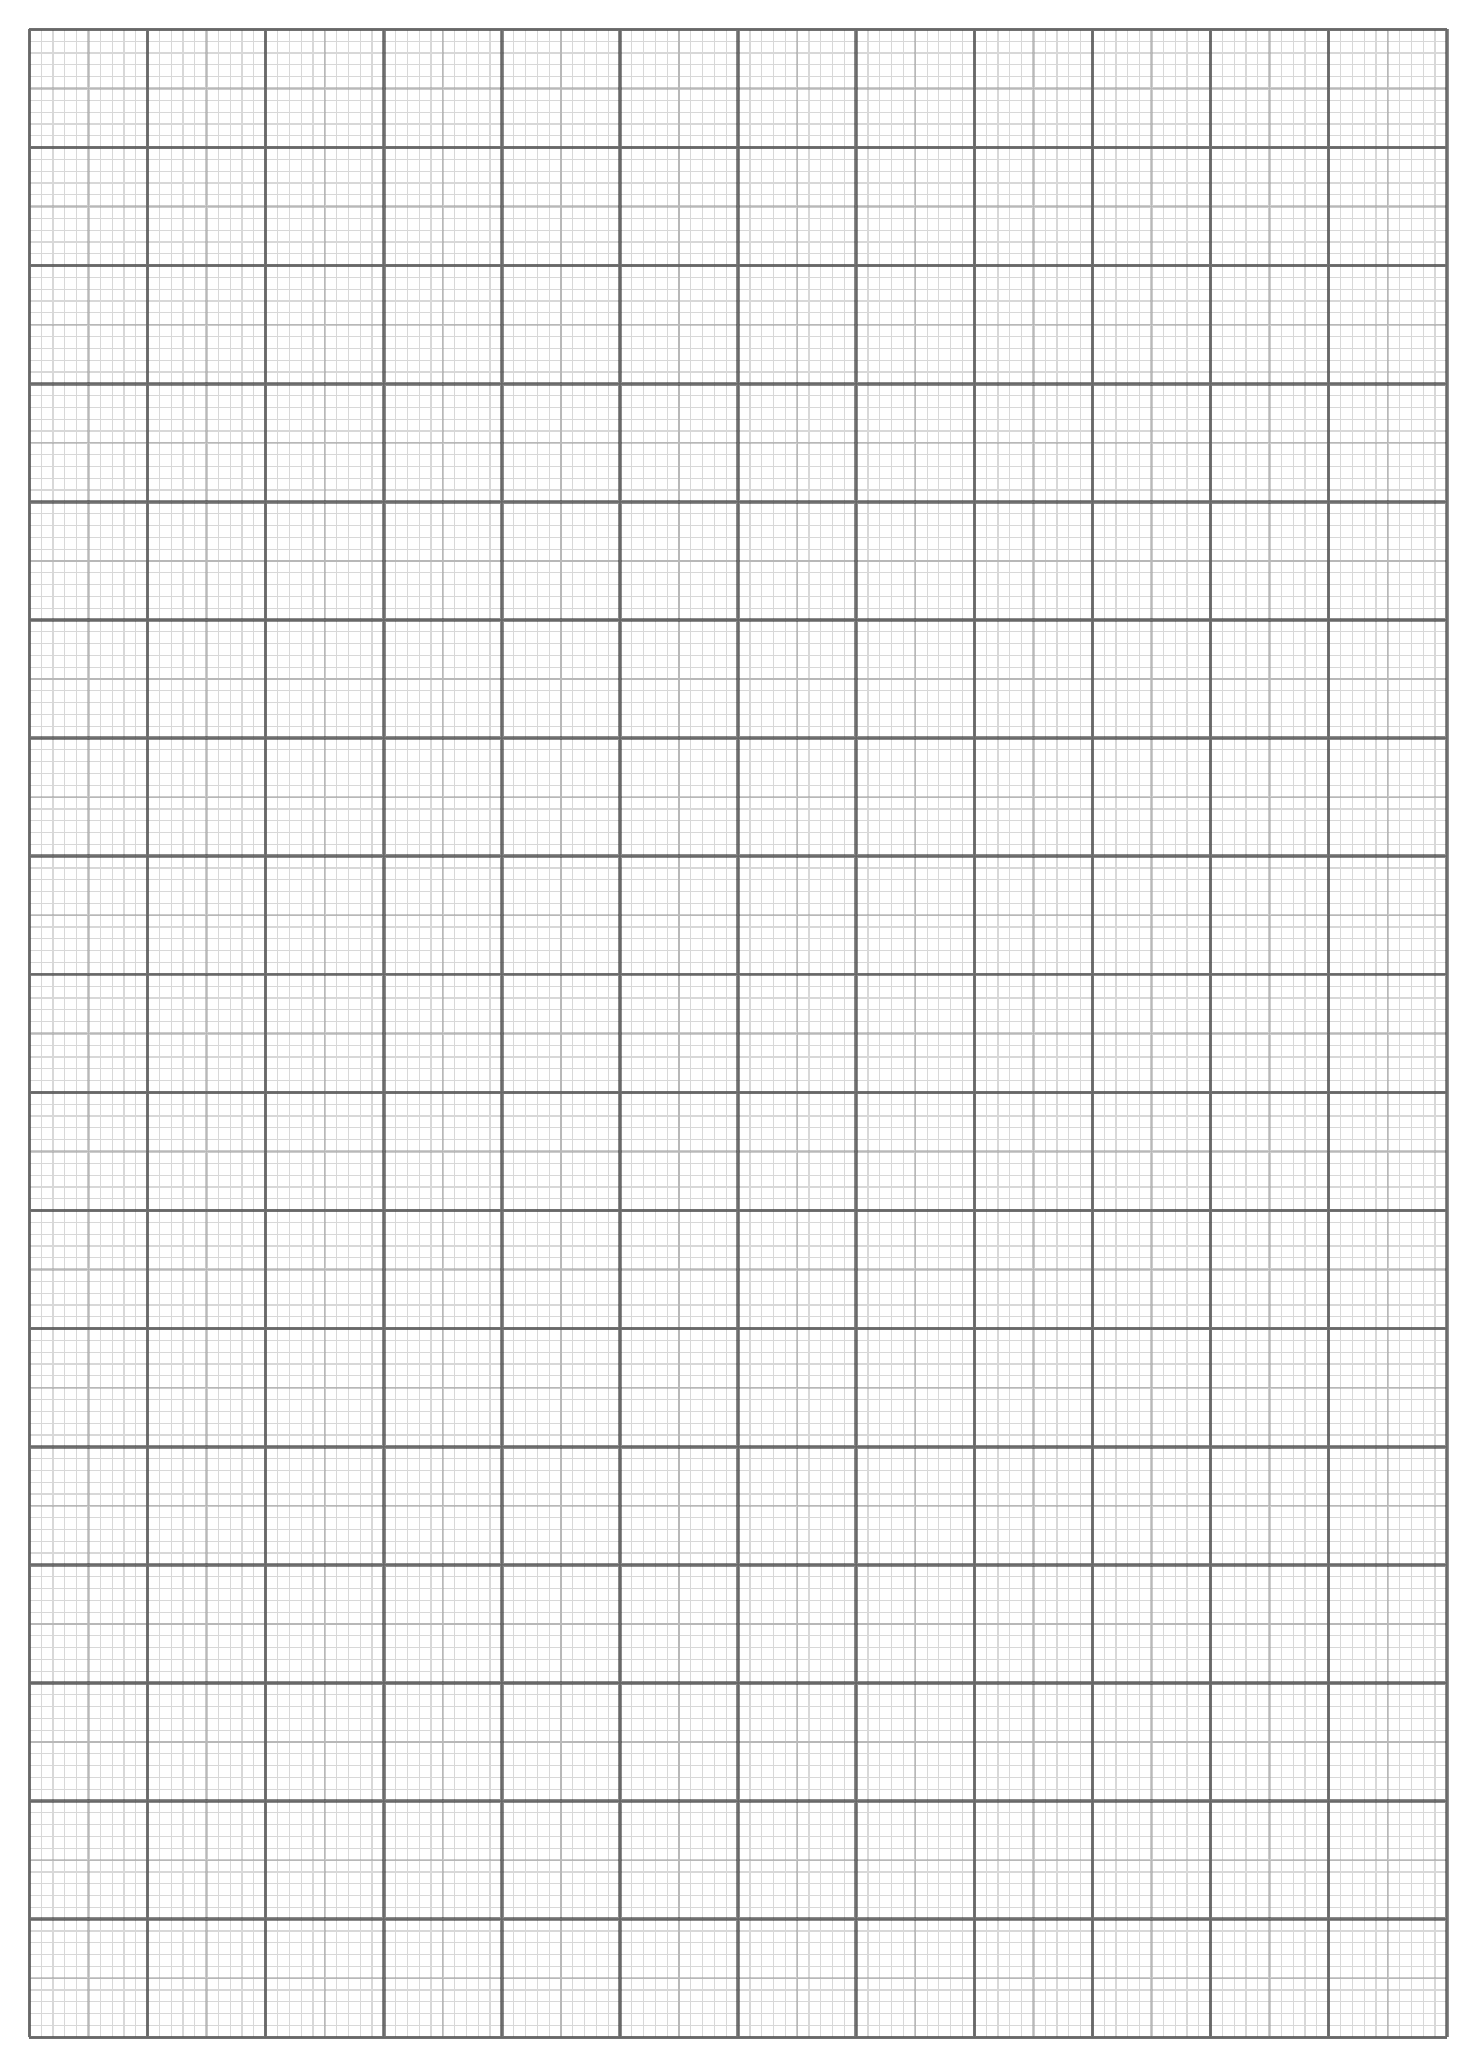
\begin{tikzpicture}[x=1cm, y=1cm, semitransparent]
  \draw[step=1\mmm, line width=0.1\mmm, black!30!white] (0,0) grid (\numberHorizontal,\numberVertical);
  \draw[step=5\mmm, line width=0.2\mmm, black!40!white] (0,0) grid (\numberHorizontal,\numberVertical);
  \draw[step=10\mmm, line width=0.3\mmm, black!90!white] (0,0) grid (\numberHorizontal,\numberVertical);
\end{tikzpicture}

\end{document}
%%% Local Variables:
%%% mode: latex
%%% TeX-master: t
%%% End: